\section{Implementierungsphase}
In dieser Phase wird detailliert beschrieben, wie die in der Entwurfsphase erarbeiteten Konzepte in ein funktionsfähiges System überführt wurden.
Der Fokus liegt dabei auf der praktischen Umsetzung der Anwendung, der Geschäftslogik sowie der Testimplementierung.
Es wird darauf geachtet, dass die Umsetzung nachvollziehbar und die Erfüllung der Projektanforderungen dokumentiert wird.

\subsection{Implementierung der Anwendung}
Nach Abschluss des Entwurfs wurde mit der eigentlichen Programmierung der Anwendung begonnen.
Dabei stand zunächst die Einrichtung der Grundstruktur im Vordergrund.

\begin{itemize}
  \item \textbf{Modularisierung:} Um eine klare Trennung der einzelnen Komponenten zu gewährleisten, wurde die Anwendung in mehrere Module unterteilt.
    Jedes Modul ist für einen spezifischen Teilbereich zuständig (z.\,B. Datenimport, Schnittstellenanbindung, Ausgabeanbindung).
  \item \textbf{Framework-Einsatz:} Die Anbindung an externe Systeme erfolgte mittels zwei zentraler Frameworks:
    \begin{itemize}
      \item \Gls{MetricQ}: Ermöglicht den Zugriff auf die Metriken und stellt sicher, dass die Anwendungsdaten aktuell und konsistent sind.
      \item \textit{pydantic}: Dieses Framework erleichtert den Umgang mit \acrlong{JSON}(\acrshort{JSON}) Daten und sorgt für eine saubere Validierung und Serialisierung der Daten.
    \end{itemize}
  \item \textbf{Technologiewahl:} Aufgrund vorhandener Erfahrungen und der hohen Entwicklungsproduktivität fiel die Entscheidung auf Python als Programmiersprache.
\end{itemize}

\noindent
Die Implementierung begann mit der Erstellung grundlegender Klassen und Funktionen.
So wurde beispielsweise die Anbindung zu \Gls{MetricQ} als ersten Schritt implementiert und eine Klasse zur Verwaltung der Konfiguration erstellt.
Diese Klasse verwendet einen sogenannten \textit{Sink}, welcher bei Änderungen der Konfiguration per Knopfdruck automatisch aktualisiert wird.
Ein exemplarischer Codeausschnitt zeigt den grundlegenden Aufbau dieser Klasse.
Weitere Details sind im Anhang unter \reference{lst:metricq_sink} zu finden, insbesondere die Methode \texttt{set\_result}.
Diese initiale Phase war entscheidend, um sicherzustellen, dass die gesamte Anwendungsarchitektur von Anfang an robust und erweiterbar gestaltet ist.

\subsection{Implementierung der Geschäftslogik}
Im Anschluss an die Einrichtung der Grundarchitektur wurde der Kern der Anwendung – die Geschäftslogik – implementiert.
Diese bildet das Herzstück des Systems, da sie für die Verarbeitung, Analyse und Weiterleitung der empfangenen Daten verantwortlich ist.

\begin{itemize}
  \item \textbf{Modulare Verarbeitung:} Die Geschäftslogik wurde in mehrere, klar abgegrenzte Module unterteilt.
    Jedes Modul übernimmt eine spezifische Funktion, etwa das Zuordnen von Checks, das Ausführen dieser oder das Überprüfen der Metriken.
  \item \textbf{Algorithmen und Entwurfsmuster:} Um die Wartbarkeit und Erweiterbarkeit zu gewährleisten, kamen bewährte Entwurfsmuster zum Einsatz.
    Beispielsweise wurde mittels \textit{Enums} die Zustandslogik vereinfacht.
    Zudem wurde das Schreiben von Daten mit Pythons \textit{yield} implementiert, was die Verarbeitung der Daten vereinfacht.
  \item \textbf{Fehlerbehandlung und Logging:} Ein robustes Fehlerhandling wurde integriert, um unerwartete Eingaben oder Systemausfälle frühzeitig zu erkennen und zu protokollieren.
    Dies erleichtert die spätere Fehlersuche und -behebung erheblich.
    Es wurde \texttt{logging} von Python verwendet, um Ereignisse zu protokollieren.
\end{itemize}

\noindent
Eine Übersicht, die ein Gesamtbild der Kommunikation zwischen den verschiedenen Komponenten der Anwendung vermittelt, kann in der \reference{fig:architecture} angesehen werden.
In dieser Darstellung ist mein Projekt als \textit{Dienstanwendung} gekennzeichnet.

\begin{figure}[H]
  \centering
  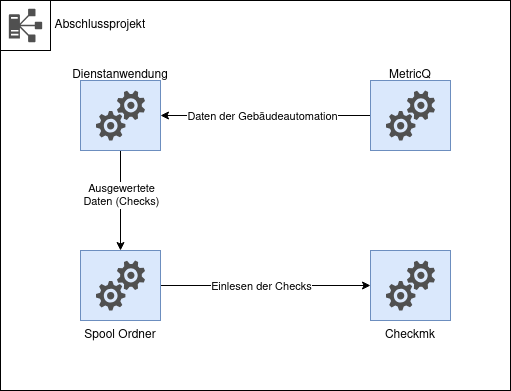
\includegraphics[width=.6\textwidth]{images/architecture.png}
  \caption{Architektur der Anwendung}
  \label{fig:architecture}
\end{figure}

\noindent
Ein konkretes Beispiel zur Darstellung eines zentralen Teils der Geschäftslogik ist die Klasse \texttt{CheckEngine}.
Diese Klasse verwaltet alle Checks und die zugehörigen \texttt{Piggyback files}.
Ein Ausschnitt der Implementierung ist im Anhang unter \reference{lst:check_engine} zu finden, und zeigt die Implementierung der \texttt{set\_result}-Methode.
Diese Klasse ist nur ein kleiner Bestandteil der gesamten Geschäftslogik, verdeutlicht jedoch den strukturierten Ansatz und die Modularität der Implementierung.

\subsection{Implementierung der Tests}
Die Qualitätssicherung ist ein wesentlicher Bestandteil des Projekts.
Bereits während der Implementierungsphase wurden umfassende Tests entwickelt, um die Funktionalität und Stabilität der Anwendung sicherzustellen.

\begin{itemize}
  \item \textbf{Unit-Tests:} Insgesamt wurden somit 35 Unit-Tests implementiert, die sich im Anhang unter \reference{lst:unit-test} zu finden befinden.
  \item \textbf{Automatisierte Testausführung:} Um die kontinuierliche Überprüfung der Softwarequalität zu gewährleisten, wurde eine CI/CD-Pipeline eingerichtet.
    Hierbei kommen moderne Tools wie \textit{GitLab CI} zum Einsatz, die bei jedem \Gls{commit} auf den \textit{main}-Branch oder einer \Gls{merge-request} automatisch die Tests ausführen.
  \item \textbf{Codequalität:} Zusätzlich wurden Linter und Codeformatierer integriert, um den Code standardkonform und wartbar zu halten.
    Dies trägt dazu bei, dass die Entwicklung konsistent und fehlerfrei verläuft.
\end{itemize}

\noindent
Die Testimplementierung sichert nicht nur die aktuelle Funktionalität, sondern ermöglicht auch eine schnelle Identifikation von Problemen bei zukünftigen Änderungen am Code.
Die wichtigsten Tests waren hierbei, die Checks für das Format der \texttt{Piggyback files} zu testen und die Implementierung der \texttt{CheckEngine} und \texttt{Check} Klassen zu testen.
Diese sind die Grundlage der Anwendung und sollten daher stets geprüft werden.

\subsection{Probleme während der Implementierungsphase}
Im Rahmen der Implementierungsphase wurde festgestellt, dass aufgrund vieler Altlasten im Bereich der Metrik-Namen Schemata die Implementierung der Anwendung schwierig wurde.
Dies hatte die Folge, dass aus den Namen keine eindeutige Identifikation der Metriken im Bezug auf die Struktur des Rechenzentrums erfolgen konnte.
Die meisten Metriken sind mit einem Namensschema definiert aus dem der Standort der Metrik bestimmt werden kann.
Zum Beispiel Informationen zum Raum oder zum Rack.
Es gibt aber auch Altlasten, welche komplett andere Namensschema verwenden.
Diese alten Namensschemata haben zum Teil keinen Standort jeglicher art in ihrem Namen.
Durch diese Probleme ist die Implementierung einer automatisierten Konfiguration der Struktur des Rechenzentrums nicht möglich gewesen.
Gemeinsam mit dem Kunden wurde entschieden, das automatisierte Erstellen der Struktur des Rechenzentrums zu streichen.
Stattdessen wurde die manuelle Konfiguration beibehalten, jedoch verbessert.
Mithilfe von sogenannten \textit{Templates} konnte der Konfigurationsaufwand reduziert werden.
Zusätzlich ermöglicht die manuelle Konfiguration jetzt die Verwendung von Labels, mit denen der Nutzer die Struktur des Rechenzentrums selbst bestimmen kann.
Diese Labels können dann in \Gls{Checkmk} als Sichten eingebunden werden.
Als Dateiformat hat der Kunde \acrshort{JSON} gewählt.

\subsection{Zusammenfassung}
Die Implementierungsphase war von einer strukturierten Vorgehensweise geprägt, die von der Einrichtung einer soliden Architektur über die detaillierte Umsetzung der Geschäftslogik bis hin zur Implementierung automatisierter Tests reichte.
Durch die konsequente Modularisierung, den Einsatz bewährter Entwurfsmuster und moderne Testmethoden konnte ein robustes und erweiterbares System realisiert werden.
